\documentclass[a4paper,12pt]{article}
\usepackage[spanish]{babel}
\usepackage[utf8]{inputenc}
\usepackage{booktabs}
\usepackage{dirtytalk}
\usepackage{graphicx}
\usepackage{makecell}

\begin{document}

\title{\Large Instituto Politécnico Nacional\\Escuela Superior de Cómputo\\Redes de Computadoras\\Tarea 1: Medios de transmisión\\Alumno: Meza Zamora Abraham Manuel}
\date{}
\maketitle

\section{Medios de transmisión}
Se le llama \textit{medio de transmisión} a todo aquello que puede llevar información de un origen a un destino. Por ejemplo, el aire es el medio de transmisión cuando dos personas tienen una conversación.\\
Las computadoras y otros medios de telecomunicaciones usan señales para representar información. Estas señales son transmitidas de un dispositivo a otro en forma de energía electromagnética, la cual es propagada a través del medio de transmisión.\\
En telecomunicaciones , los medios de transmisión se pueden clasificar en dos categorías: guiados y no guiados.

\begin{figure}[h]
\centering
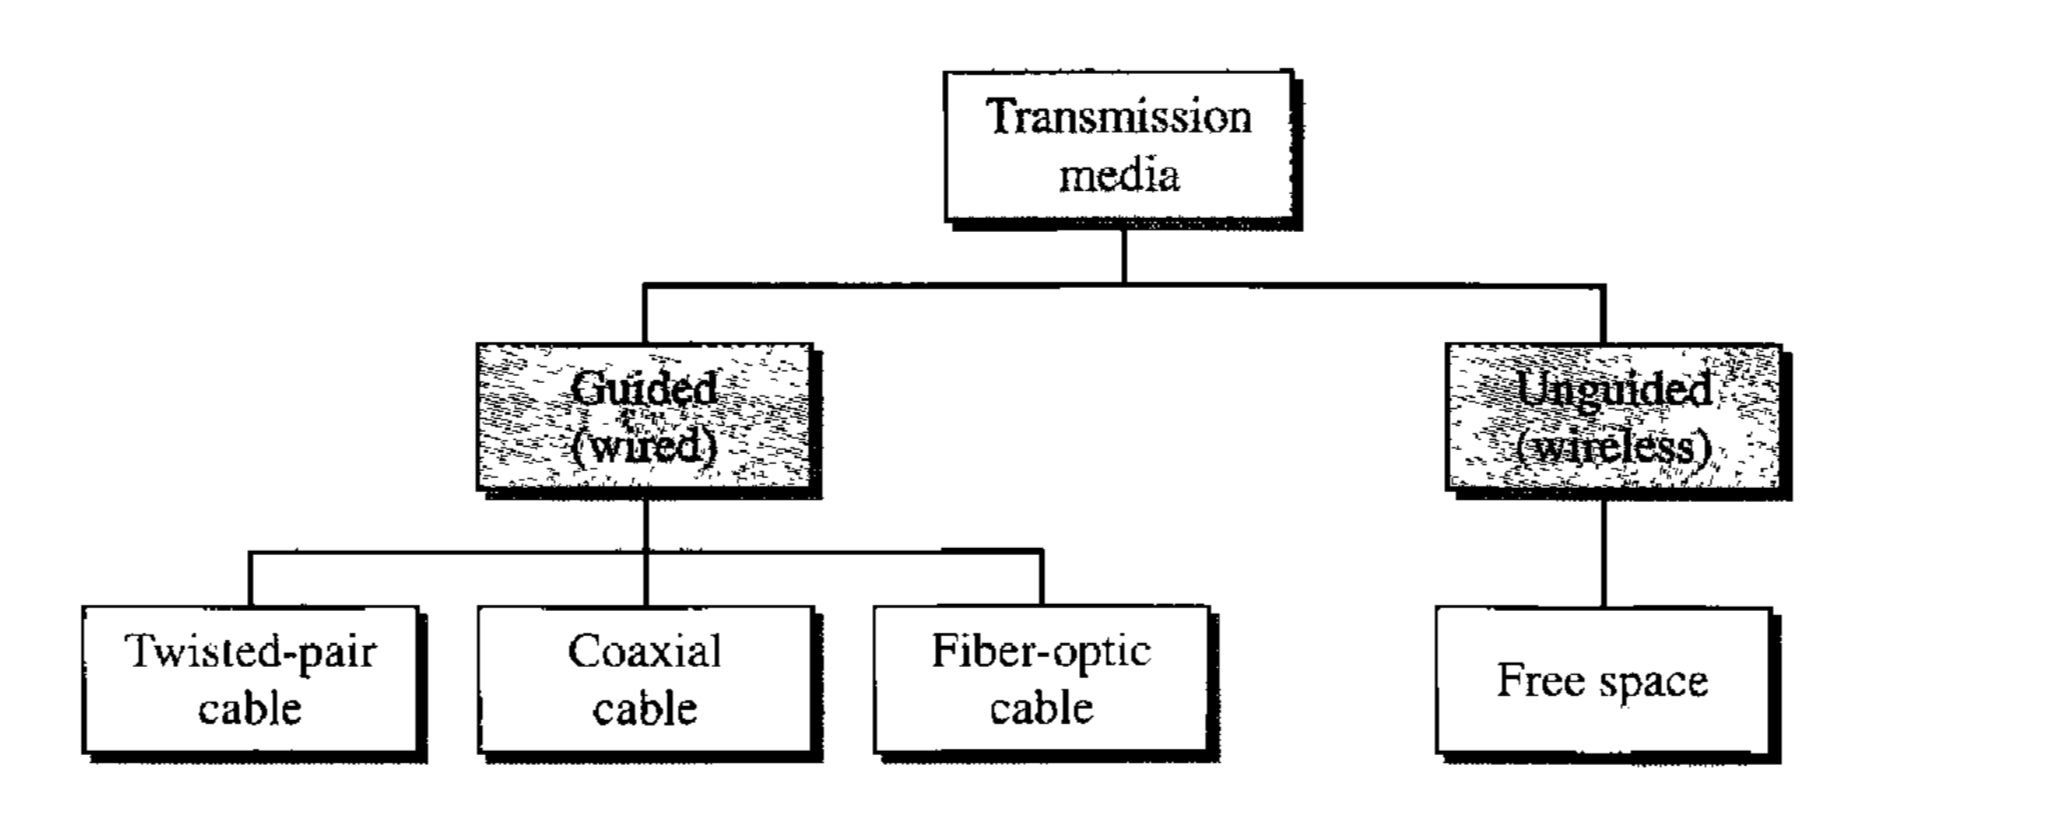
\includegraphics[width=0.75\textwidth]{figuno}
\caption{Clasificación de los medios de transmisión.}
\label{ene}
\end{figure}

\section{Medios guiados}
Los medios de transmisión guiados son aquellos que proveen algún tipo de conducto de un dispositivo a otro, como un cable coaxial y la fibra óptica entre otros. La señal que viaja a través de estos medios está dirigida y contenida por los límites físicos del medio.

\begin{figure}[h]
\begin{center}
\begin{tabular}{| c | c  | c | c | }
\hline
 \textbf{Categoría} & \textbf{Ancho de banda} & \textbf{Velocidad	} & \textbf{Distancia}\\ 
 \hline
Categoría 1 & 0.4 MHz & 100 Kbps & 100 m\\ 
 \hline
Categoría 2 & 4 MHz & 4 Mbit/s & 100 m\\ 
 \hline
Categoría 3 & 16 MHz & 10 Mbit/s & 100 m\\ 
 \hline
Categoría 4 & 20 MHz & 16 Mbit/s & 100 m\\ 
 \hline
Categoría 5/5e& 100 MHz & 1000 Mbps & 100 m\\ 
 \hline
Categoría 6 & 250 MHz & 1 Gbps & 90 m\\ 
 \hline
Categoría 6 & 550 MHz & 10 Gbit/s & 100 m\\ 
\hline
Categoría 7/7a & 600 - 1200 MHz & 10 Gbit/s  & 100 m \\
\hline
Coaxial grueso & 350 GHz & 10 Mb/s & 500 m \\
\hline
Coaxial fino & 350 GHz  & 10 Mb/s  & 185 m \\
\hline
Fibra óptica monomodo  & 100 GHz  & 622 Mbps & 100 Km \\
\hline
Fibra óptica multimodo & 500 GHz  & 10 - 155 Mbps & 2.4 Km \\
\hline
\end{tabular}
\caption{Tabla comparativa de medios de transmisión guiados}
\end{center}
\end{figure}

\section{Medios no guiados}
Los medios de transmisión no guiados transportan ondas electromagnéticas sin utilizar un conductor físico. A este tipo de comunicación también se le conoce como \textit{comunicación inalámbrica}. Generalmente las señales son transmitidas en un espacio libre por lo que se encuentran disponibles a todos los que tengan un dispositivo capaz de recibirlas.

\begin{figure}[h]
\centering
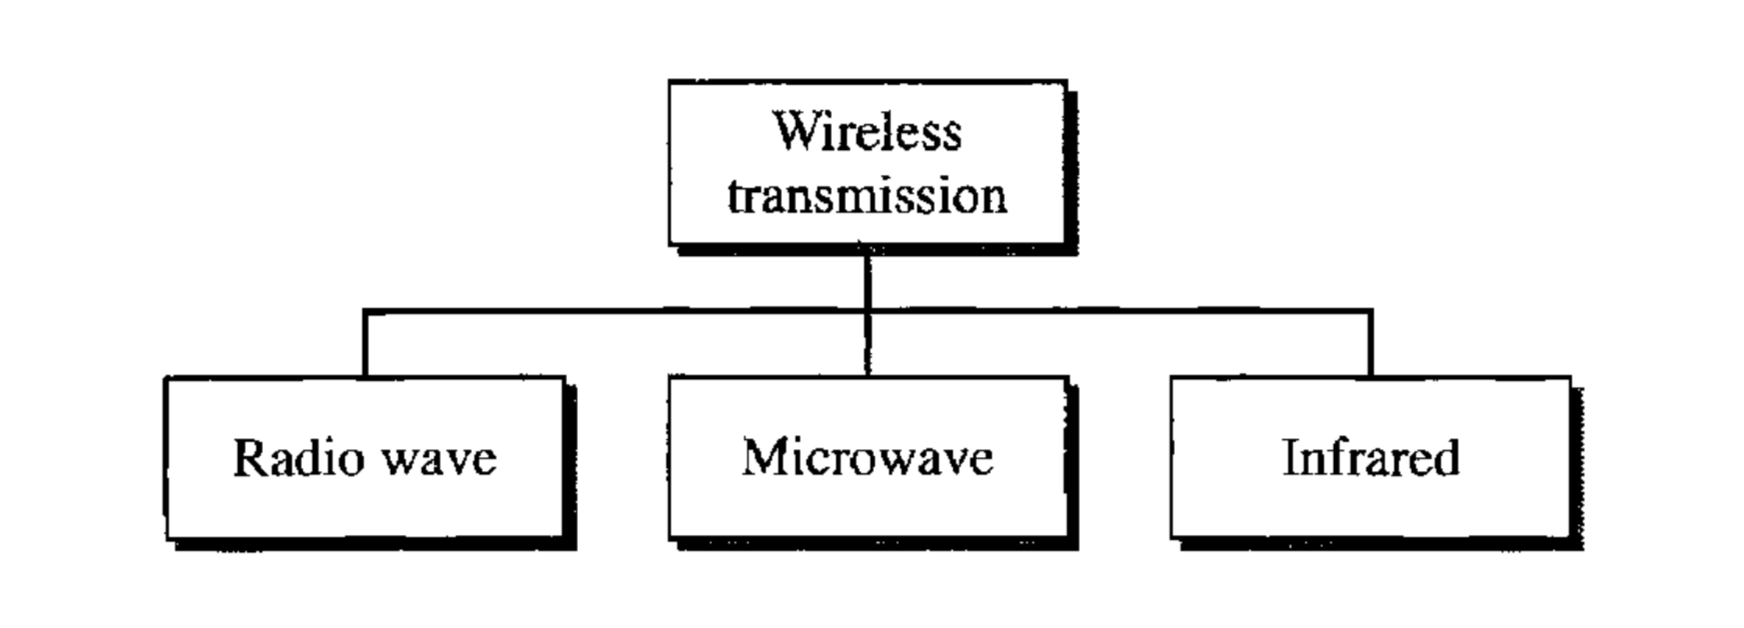
\includegraphics[width=0.60\textwidth]{figdos}
\caption{Clasificación de los medios de transmisión.}
\label{ene}
\end{figure}

\begin{figure}[h]
\begin{center}
\begin{tabular}{| c | c  | c | c | }
\hline
 \textbf{Categoría} & \textbf{Ancho de banda} & \textbf{Velocidad	} & \textbf{Distancia}\\ 
 \hline
 Microondas terrestres & 2 - 40 GHz & 500 Mbps & 7.14 Km \\
  \hline
 Microondas satelitales & 1 - 10 GHz & 275 MGbps & 10 Km \\
  \hline
 Infrarrojo & 300 GHz hasta 400 THz & 115 Kbps & 3 - 5 m \\
  \hline
 Ondas cortas & 3 - 30 MHz & 300.000 Km/s & 10 - 100 m \\
  \hline
 Ondas de luz & 100 - 400 MHz & 300.000 Km/s  & 500 m \\
 \hline
\end{tabular}
\caption{Tabla comparativa de medios de transmisión no guiados  }
\end{center}
\end{figure}


\begin{thebibliography}{12}
\bibitem{Libro} 
Behrouz A. Forouzan. (2007). DATA COMMUNICA TIONS AND NETWORKING. USA: McGraw-Hill.

\bibitem{wikipedia}
García Teodoro, Pedro; Díaz Verdejo, Jesús Esteban; López Soler, Juan Manuel (2003). Transmisión de datos y redes de computadores. Pearson Educación.

 
\end{thebibliography}

\end{document}